\documentclass[a4paper]{article}
% \documentclass{proc}

\usepackage{a4}
\usepackage{lipsum}
\usepackage{graphicx}
\usepackage{float}
\usepackage{listings}
\usepackage{color}
\usepackage{hyperref}
\usepackage{cite}
\usepackage{textgreek}
\usepackage{amsfonts}

\usepackage[margin=1.25in]{geometry}

\date{}

\title{A Review of Adversarial Neural Cryptography}
\author{
  {\bf Alisamar Husain}\\
  Dept. of Electrical Engineering\\
  Jamia Millia Islamia
}

\begin{document}
  \maketitle

  \begin{abstract}
    Artificial neural networks are well known for their ability to selectively 
    explore the solution space of a given problem.
    One of the recent applications of this feature is in the field of neural 
    cryptography, which provides an opportunity to use ANNs to encrypt data 
    such that it cannot be decrypted by an attacker.

    In this paper we examine the efficacy, feasibility and 
    general practicality of the use of {\it adversarial neural cryptography}, 
    as coined by Abadi et al. in \cite{seminalanc}, and neural cryptography
    in general. We test systems recommended in the literature and examine their 
    use in data transmission systems for the purpose of encrypting data from
    the perspective of securing a communication channel.
  \end{abstract}
 
  \section{Introduction}
  The field of cryptography is broadly concerned with algorithms and protocols 
  that ensure the secrecy and integrity of information. Cryptographic mechanisms are 
  typically described as programs or Turing machines. By this definition, an
  appropriate neural network can possibly be considered a cryptographic function.

  As neural networks are applied to increasingly complex tasks, they are often trained to meet end-to-end 
  objectives that go beyond simple functional specifications. These objectives include, for
  example, generating realistic images\cite{gans} and solving multiagent problems. 

  Cryptography is broadly concerned with algorithms and protocols that ensure the secrecy and integrity
  of information. Cryptographic mechanisms are typically described as programs or Turing
  machines. Attackers are also described in those terms, with bounds on their complexity 
  and on their chances of success. A mechanism is deemed secure if it achieves its goal 
  against all attackers. For instance, an encryption algorithm is said to be secure if 
  no attacker can extract information about plaintexts from ciphertexts.
  Modern cryptography provides rigorous versions of such definitions.

  Neural networks are generally not meant to be great at cryptography. Famously, the simplest neural
  networks cannot even compute XOR, which is basic to many cryptographic algorithms. Nevertheless,
  as was demonstrated in the seminal paper on this subject\cite{seminalanc} by Abadi et. al in 2016,
  neural networks can learn to protect the confidentiality of their data from
  other neural networks: they discover forms of encryption and decryption, without being taught 
  specific algorithms for these purposes.

  Knowing how to encrypt is seldom enough for security and privacy. Interestingly, neural networks
  can also learn what to encrypt in order to achieve a desired secrecy property while maximizing
  utility. Thus, when we wish to prevent an adversary from seeing a fragment of a plaintext, or from
  estimating a function of the plaintext, encryption can be selective, hiding the plaintext only partly.

    \subsection{Terminology}
    Certain terms are frequently used while talking about cryptographic mechanisms
    and it is beneficial to have an understanding of what these refer to. Some
    of these will be used in this paper to commonly identify certain parts of the 
    system and some are abbreviations made for convenience.

    A {\bf party} is a machine, or actor in general, which is using a communication
    channel to communicate with another machine. There are two major types of parties
    which we are concerned with, {\bf participants and attackers.}
    
    A {\bf participant} is a party which actively takes part in the communication and
    sends messages on the channel. The goal of encryption is to ensure that the 
    communication between any two parties can only be intercepted and understood 
    by them.

    An {\bf attacker} is a party which attempts to intercept and understand the
    communication between two participants.
  
  \paragraph{Attackers}
  Attackers are also described in those terms, with bounds on their complexity 
  (e.g., limited to polynomial time) and on their chances of success 
  (e.g., limited to a negligible probability). A mechanism is deemed secure if 
  it achieves its goal against all attackers. For instance, an encryption
  algorithm is said to be secure if no attacker can extract information about 
  plaintexts from ciphertexts.
  Modern cryptography provides rigorous versions of such definitions, like those 
  given by Goldwasser \& Micali. \cite{Goldwasser}
  
    \subsection{Symmetric Encryption}
    Symmetric-key cryptography refers to encryption methods in which both the sender and 
    receiver share the same key (or, less commonly, in which their keys are different, but 
    related in an easily computable way).

    Symmetric key ciphers are implemented as either block ciphers or stream ciphers. 
    A block cipher enciphers input in blocks of plaintext as opposed to individual characters, 
    the input form used by a stream cipher.

    \subsection{Adversarial Neural Cryptography}
    This section discusses how to protect the confidentiality of plaintexts using shared keys. It describes
    the organization of the system that we consider, and the objectives of the participants in this system.
    It also explains the training of these participants, defines their architecture, and presents experiments.

    A classic scenario in security involves three parties: Alice, Bob, and Eve. Typically, Alice and Bob
    wish to communicate securely, and Eve wishes to eavesdrop on their communications. Thus, the
    desired security property is secrecy (not integrity), and the adversary is a “passive attacker” that
    can intercept communications but that is otherwise quite limited: it cannot initiate sessions, inject
    messages, or modify messages in transit.

      \subsubsection{Mathematical Background}
      We write $A(\Phi_{A}, P,K)$ for Alice’s output on input $P,K$, write $B(\Phi_{B},C,K)$ for Bob’s output on
      input $C,K$, and write $E(\Phi_{E},C)$ for Eve’s output on input $C$. We introduce a distance function d on
      plaintexts.  
      
      Although the exact choice of this function is probably not crucial, for concreteness we
      take the L1 distance 
        
      \[ d(P, P^\prime) = \Sigma_{i=1}^N | P_{i} - P_{i}^\prime | \]
      
      where N is the length of plaintexts. 
      We define a per-example loss function for Eve.
      Intuitively this represents how much Eve is wrong when the plaintext is P and the
      key is K. We also define a loss function for Eve over the distribution on plaintexts and keys by
      taking an expected value:

      \[ L_{E}(\Phi_{A}, \Phi_{E}) = \mathbb{E}_{P,K} [ d(P, E(\Phi_{E}, A(\Phi_{A},  P, K))) ] \]

      We obtain the “optimal Eve” by minimizing this loss:
      
      \[ O_{E}(\theta_{A}) = argmin_{\theta_{E}}(L_{E}(\theta_{A}, \theta_{E})) \]

      Similarly, we define a per-example reconstruction error for Bob, and extend it to the 
      distribution on plaintexts and keys. We define a loss function for Alice and Bob by 
      combining $L_{B}$ and the optimal value of $L_{E}$:
      
      \[ L_{AB}(\Phi_{A}, \Phi_{E}) = L_{B}(\Phi_{A}, \Phi_{B}) - L_{E}(\Phi_{A}, O_{E}(\theta_{A})) \]
      
      This combination reflects that Alice and Bob want to minimize Bob’s reconstruction error and to
      maximize the reconstruction error of the “optimal Eve”. The use of a simple subtraction is somewhat
      arbitrary; below we describe useful variants. We obtain the “optimal Alice and Bob” by minimizing
      
      \[ (O_{A}, O_{B}) = argmin_{(\theta_{A}, \theta_{B})}(L_{AB}(\theta_{A}, \theta_{B})) \]
      
      We write “optimal” in quotes because there need be no single global minimum. In general, there
      are many equi-optimal solutions for Alice and Bob. As a simple example, assuming that the key is
      of the same size as the plaintext and the ciphertext, Alice and Bob may XOR the plaintext and the
      ciphertext, respectively, with any permutation of the key, and all permutations are equally good as
      long as Alice and Bob use the same one; moreover, with the way we architect our networks (see
      Section 2.4), all permutations are equally likely to arise.
    

  
  \section{Related Work}
  
  \pagebreak
  \section{Methodology}
  We use a simple setup in order to build and test the networks. The models are 
  first implemented using the Python programming language and after obtaining a 
  suitably trained and validated model, we can move on to testing. 

    \subsection{Network Architecture} \label{sec:anc_netarch}
    The Architecture of Alice, Bob, and Eve Because we wish to explore whether a general neural
    network can learn to communicate securely, rather than to engineer a particular method, we aimed
    to create a neural network architecture that was sufficient to learn mixing functions such as XOR,
    but that did not strongly encode the form of any particular algorithm.
    To this end, we chose the following “mix \& transform” architecture. It has a first fully-connected
    (FC) layer, where the number of outputs is equal to the number of inputs. The plaintext and key
    bits are fed into this FC layer. Because each output bit can be a linear combination of all of the
    input bits, this layer enables—but does not mandate—mixing between the key and the plaintext bits.
    In particular, this layer can permute the bits.

    \begin{figure}[H]
      \centering
      \includegraphics[width=\textwidth]{../ref/anclayers.png}
      \caption{Modified network Model from Abadi et al.}
      \label{fig:anclayers}
    \end{figure}
    
    The FC layer is followed by a sequence of convolutional
    layers, the last of which produces an output of a size suitable for a plaintext or ciphertext.
    These convolutional layers learn to apply some function to groups of the bits mixed by the previous
    layer, without an a priori specification of what that function should be. Notably, the opposite order
    (convolutional followed by FC) is much more common in image-processing applications. Neural
    networks developed for those applications frequently use convolutions to take advantage of spatial
    locality.  
      
    For neural cryptography, we specifically wanted locality—i.e., which bits to combine—to
    be a learned property, instead of a pre-specified one. While it would certainly work to manually pair
    each input plaintext bit with a corresponding key bit, we felt that doing so would be uninteresting.
    We refrain from imposing further constraints that would simplify the problem. For example, we do
    not tie the parameters $\Phi_{A}$ and $\Phi_{B}$, as we would if we had in mind that Alice and Bob should both
    learn the same function, such as XOR.

    \subsection{Training Parameters}
    The parameters which aren't learnt by the network but directly affect the performance are
    called {\bfseries hyperparameters}. These are important since the right choice of hyperparameters
    can get us to the optimal model very quickly.

    For our purposes the important parameters are the {\bfseries key length, learning rate and the
    loss coefficients} in calculation of the loss for Alice and Bob. Various combinations are tried
    until one good set of values is obtained by experimentation.

    % The following table lists the various values of the hyperparameters that were tried and
    % produced some useful results.

    \begin{center}
      \begin{tabular}{ c|c|c }
        \textbf{Key Size} & \textbf{Learning Rate} & \textbf{Weight Decay} \\
        4 bits            & 0.0002                 & 0.000001              \\
        8 bits            & 0.0004                 & 0.000002              \\
        16 bits           & 0.0008                 &                       \\
        32 bits           &                        &                       \\
      \end{tabular}
    \end{center}

    \subsection{Tools Used}
    The models are implemented using PyTorch, a popular framework for building
    neural networks in Python. The models are built per the specification given in
    the literature and trained with the help of several common Python libraries.
    We use Tensorboard to monitor the training process and log the training metadata.

  \section{Results}
  After training the networks suitably, they are put through the validation procedure to test their
  efficacy with unseen new data. The models that meet a reasonable level of validation accuracy are
  considered to have converged and thus a success.

  \subsection{ANC}
  The following figures show the loss trends for the ANC model with and without the adversary.
  We can see the loss decreasing fast without the adversary but when the eavesdropper is introduced,
  the loss still decreases. This is a sign that the cryptosystem is working \cite{perfanc}.

  \begin{figure}[H]
    \centering
    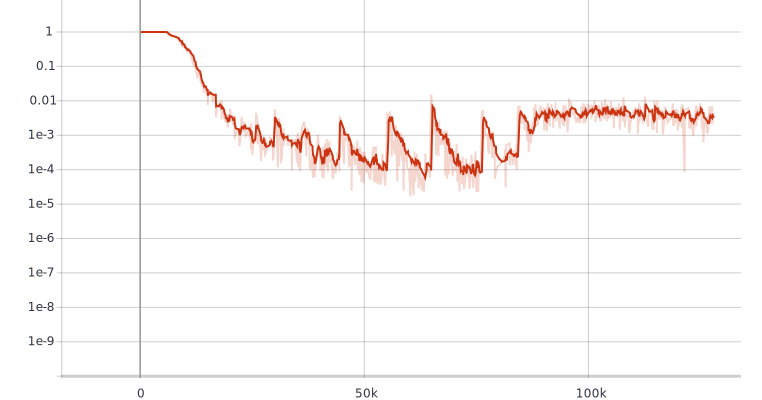
\includegraphics[height=1.5in]{../../models/anc/graphs/Loss_Training.png}
    \caption{Training Loss Trend with ANC}
    \label{fig:trn_crnet}
  \end{figure}

  \begin{figure}[H]
    \centering
    \includegraphics[width=0.48\textwidth]{../../models/cryptonet/graphs/loss_1E64x256v17.png}
    \includegraphics[width=0.48\textwidth]{../../models/anc/graphs/loss_1E2000v6.png}
    \caption{Loss Trend with ANC model by Abadi et al.}
    \label{fig:res_anc}
  \end{figure}

  \begin{center}
    \begin{tabular}{ c c c c }
      \hline
      \textbf{Key Size} & \textbf{Learning Rate} & \textbf{Epochs} & \textbf{Convergence} \\ \hline
      8 bits            & 0.0008                 & 8               & 4/10                 \\
      16 bits           & 0.0008                 & 10              & 4/10                 \\
      16 bits           & 0.0010                 & 16              & 6/10                 \\
      \hline
    \end{tabular}
  \end{center}
    
  The table above shows the number of times out of 10, that the networks converged with a 
  reasonable validation accuracy with different hyperparameters in the training.\\

  \subsection{Cryptonet}
  The following figures show the loss trends for the Cryptonet model with and without the adversary.
  Immediately we can notice that the rate of decrease of the loss is slower, which is a clear sign that
  the adversary Eve is having an effect on the training of Alice and Bob.

  \begin{figure}[H]
    \centering
    \includegraphics[height=1.5in]{../../models/cryptonet/graphs/TrainingLoss[S].png}
    \caption{Training Loss Trend with Cryptonet}
    \label{fig:trn_crnet}
  \end{figure} 

  \begin{figure}[H]
    \centering
    \includegraphics[width=0.48\textwidth]{../../models/cryptonet/graphs/loss_1E64x256v13.png}
    \includegraphics[width=0.48\textwidth]{../../models/cryptonet/graphs/loss_1E64x256v19.png}
    \caption{Loss Trend with Cryptonet model by Coutinho et al.}
    \label{fig:res_crnet}
  \end{figure}

  \begin{center}
    \begin{tabular}{ c c c c }
      \hline
      \textbf{Key Size} & \textbf{Learning Rate} & \textbf{Epochs} & \textbf{Convergence} \\ \hline
      4 bits            & 0.0008                 & 8               & 2/10                 \\
      8 bits            & 0.0008                 & 10              & 4/10                 \\
      8 bits            & 0.0008                 & 16              & 5/10                 \\
      \hline
    \end{tabular}
  \end{center}
  
  \section{Conclusions}

  \bibliographystyle{IEEEtran}
  \bibliography{../../resources/citations}
\end{document}
